%%% Laboratory	 Notes
%%% Template by Mikhail Klassen, April 2013
%%% Contributions from Sarah Mount, May 2014
\documentclass[a4paper]{tufte-handout}

\newcommand{\workingDate}{\textsc{Fall $|$ 2016}}
\newcommand{\userName}{Cail Daley}
\newcommand{\institution}{Wesleyan University}

\usepackage{aumic_notes}


\usepackage{hyperref}
\usepackage{hypcap}
\hypersetup{
    pdffitwindow=false,            % window fit to page
    pdfstartview={Fit},            % fits width of page to window
    pdftitle={HD_100546_Modeling_Notes},     % document title
    pdfauthor={Cail Daley},         % author name
    pdfsubject={},                 % document topic(s)
    pdfnewwindow=true,             % links in new window
    colorlinks=true,               % coloured links, not boxed
    linkcolor=DarkScarletRed,      % colour of internal links
    citecolor=DarkChameleon,       % colour of links to bibliography
    filecolor=DarkPlum,            % colour of file links
    urlcolor=DarkSkyBlue           % colour of external links
}

\title{AU Mic Notes}
\date{2016}

\begin{document}
\maketitle

\textbf{Note: I've switched to Markdown for ease of note taking. Please refer to aumic\_notes.md for work after 23 January.}
%%%%%%%%%%%%%%%%%%%%%%%%%%%%%%%%%%%%%%%%%%%%%%%%%%%%%%%%

\begin{tasks}
	\begin{itemize}
		\item Write up :/
	\end{itemize}
\end{tasks}

%%%%%%%%%%%%%%%%%%%%%%%%%%%%%%%%%%%%%%%%%%%%%%%%%%%%%%%%

\begin{maybe}
	\begin{itemize}
		\item
	\end{itemize}
\end{maybe}

%%%%%%%%%%%%%%%%%%%%%%%%%%%%%%%%%%%%%%%%%%%%%%%%%%%%%%%%

\begin{mer}
	\begin{itemize}
		\item
	\end{itemize}

\end{mer}
%%%%%%%%%%%%%%%%%%%%%%%%%%%%%%%%%%%%%%%%%%%%%%%%%%%%%%%%

\newday{23 January 2017}
Checking noise statistics for natural clean:\\
\begin{itemize}
  \item image area $\approx$ 15x15 $\to$ 225 arcsec
  \item beam area $\approx$ 0.65 arcsec --> $\sim$ 346 beams in image
  \item 2$\sigma$ 5\% $\to 0.05 * 346 = 17$
  \item found about 19 beams
\end{itemize}

\noindent Checking noise statistics for natural clean with 200klam taper:\\
\begin{itemize}
  \item image area $\approx$ 15x15 $\to$ 225 arcsec
  \item beam area $\approx$ 1.93 arcsec --> $\sim$ 117 beams in image
  \item 2$\sigma$ 5\% $\to 0.05 * 346 = 6$
  \item found about 9 beams
\end{itemize}
%%%%%%%%%%%%%%%%%%%%%%%%%%%%%%%%%%%%%%%%%%%%%%%%%%%%%%%%

\newday{13 January 2017}
AU Mic was observed on three dates with ALMA: 26 March 2014, 18 August 2014, and 24 June 2015. All observations were configured with four spectral windows, and employed ALMA's 12 m antennas and Band 7 receivers. One spectral window was centered around the CO $J = (2-1)$ transition at a frequency of 230.538001 Ghz, while the remainging three were configured to detect continuum emission with maximum bandwidths of 2 Ghz and channel spacing of 15.6 Mhz. Central frequencies for the continuum bands are 228.5, 213.5, and 216.0 Ghz.

The 26 March data were obtained with 32 antennas and baselines ranging between  14 and 437 m; weather conditions were excellent ($\sim$0.6 mm of precipitable water vapor). The quasar J1924-2914 was used as a bandpass calibrator, and Titan was used to calibrate absolute flux. After these initial calibrations, observations cycled every seven minutes between AU Mic and the quasar J2101-2933, which was used for phase calibration. In total, 35 minutes were spent on source.

The 18 August utilized 35 antennas in a more extended antenna configuration (baselines between 20 and 1268 m) to probe the small scale structure of the disk. Weather conditions were poor, with $\sim$1.6 mm of precipitable water vapor. The quasars J2056-4714 (bandpass calibration) and J2056-472 (absolute flux calibration) were observed at the beginning of the observation window. For the remainder of the time block antennas cycled between seven-minute observations of AU Mic and brief observations of the quasars J2101-2933, for phase calibration, and J2057-3734, to test the quality of the gain transfer. AU Mic was observed for 35 minutes altogether.

The 24 June observation was taken to supplement the 18 August's, which was of poor quality due to weather conditions? 37 antennas covered baselines from 30 to 1431 m and weather conditions were good-- 0.7 mm of precipitable water vapor. Bandpass and absolute flux calibrations, making use of J1924-2914 and Titan respectively, were conducted at the beginning of the scheduled time block. Short observations of the quasars J2056-3208 for phase calibration and J2101-2933 to assess the quality of the gain transfer were interspersed among seven-minute observations of the source, which was observed for 33 minutes. The central star flared during the last observation of AU Mic, from 04:23:38-04:29:58.

Calibration, reduction, and imaging were carried out using the CASA and MIRIAD software packages. Standard ALMA reduction scripts were applied to the datasets: phase calibration was accomplished via water vapor radiometry tables, and system temperature calibrations were performed to account for variations in instrument and weather conditions. Flux and bandpass calibrations were subsequently applied.

The authors travelled to the NRAO facility in Charlottesville, VA in October 2015 to further process the data; in particular the trip was intended to allow on-site correction of the 24 June flare. Tasks used to reduce the data at the NRAO facility were are part of the CASA package. First, weights were assigned to all datasets using the task \textit{initweights}. An elliptical gaussian was then fit to the disk and star in the image plane of each dataset using the task \textit{imfit}; the equatorial coordinates of the the best fit gaussian peak were then used to phase shift the dataset via the task \textit{fixvis} to account for AU Mic's proper motion. \footnote{Should I put the derived phase centers in a table?}

Task order?
\begin{itemize}
  \item initweights
  \item imfit (small box in center)
  \item split to human-comprehensible name
  \item fixvis
  \item for non-flare dates:
  \begin{itemize}
    \item cl, ft with imfit peak OR
    \item cl, ft with uvmodelfit spw mean (We DID use this)
  \end{itemize}
  \item for flare/June dates:
  \begin{itemize}
    \item cl, ft with uvmodelfit spw mean
  \end{itemize}
  \item split to add .uvsub--seems like it should be the same file?
\end{itemize}





Flare time--4:23:38-4:29:58

\begin{table}
	\label{tab:flare fluxes}
	\caption{Subtracted point-source fluxes}
	\begin{tabu} to \textwidth {X[l]X[r]}
		\toprule
		Time (UTC) & Point-source Flux ($\mu$Jy) \\
		\midrule
    03:45:0-04:20:0 (no flare) & ($4.1 \pm 0.2)  \times 10^2$\\
		4:23:38-4:24:00 & $(9.2 \pm 1.7) \times 10^2$ \\
		4:23:38-4:24:00 & $(1.146 \pm 0.010) \times 10^4$ \\
		4:25:00-4:26:00 & $(3.59 \pm 0.10) \times 10^3$ \\
		4:26:00-4:27:00 & $(1.58 \pm 0.10) \times 10^3$ \\
		4:27:00-4:28:00 & $(4.50 \pm 1.0) \times 10^2$ \\
		4:28:00-4:29:00 & $(4.60 \pm 1.0 \times 10^2$ \\
		4:29:00-4:29:58 & $(5.20 \pm 1.0) \times 10^2$\\
		\bottomrule
	\end{tabu}
\end{table}



\begin{itemize}
	\item 18 aug
	      \begin{itemize}
	      	\item PWV roughly 1.6mm
	      	\item Objects:
	      	      \begin{itemize}
	      	      	\item AU Mic: around 6m per observation, 5 observations
	      	      	\item J2056-4714: bandpass calibrator, observed for \abt 5 min at beginning
	      	      	\item J2056-472: amplitude calibrator, observed for \abt 3 min at beginning
	      	      	\item J2101-2933: phase calibrator, observed for \abt 1 m each, 4 times
	      	      	\item J2057-3734: delay calibrator, observed for \abt 1 m each, 4 times
	      	      \end{itemize}
	      	\item spws:
	      	      \begin{itemize}
	      	      	\item 0: ctr=230.538 Ghz, totBW=1875000 khz, chanwid=488 kHz
	      	      	\item 1: ctr=228.492 Ghz, totBW=2e6 khz, chanwid=15625 khz
	      	      	\item 1: ctr=213.492 Ghz, totBW=2e6 khz, chanwid=-15625 khz
	      	      	\item 1: ctr=215.992 Ghz, totBW=2e6 khz, chanwid=-15625 khz
	      	      \end{itemize}
	      	\item 35 antennas-- 12 m diameter
	      	\item baselines between 20 and 1268
	      	\item 5:18:14 to 5:33:22, 5:38:12 to 5:53:20 2106 seconds
          \item History:
          \begin{itemize}
            \item applycal: phase, delay, target; tsyscal, wvrcalflag
            \item applycal: flux, amplitude, bandpass; same tables?
          \end{itemize}
	      \end{itemize}

	\item 26 mar
	      \begin{itemize}
	      	\item \abt .6mm pwv
	      	\item Objects:
	      	      \begin{itemize}
	      	      	\item J1924-2914: bandpass calibrator, observed for \abt 5 min at beginning
	      	      	\item Titan: amplitude calibrator, observed for \abt 3 min at beginning
	      	      	\item J2101-2933: phase calibrator, observed for \abt 1 m each, 6 times
	      	      	\item AU Mic: \abt 7m per observation, 5 observations
	      	      \end{itemize}
	      	\item spws:
	      	      \begin{itemize}
	      	      	\item 0: ctr=230.564 Ghz, totBW=1875000 khz, chanwid=488 kHz
	      	      	\item 1: ctr=228.519 Ghz, totBW=2e6 khz, chanwid=15625 khz
	      	      	\item 1: ctr=213.518 Ghz, totBW=2e6 khz, chanwid=-15625 khz
	      	      	\item 1: ctr=216.018 Ghz, totBW=2e6 khz, chanwid=-15625 khz
	      	      \end{itemize}
	      	\item 32 antennas-- 12 m diameter
	      	\item baselines between 15 and 437
	      	\item 9:41:54 to 10:16:56 2102 seconds
	      \end{itemize}

	\item 24 jun
	      \begin{itemize}
	      	\item \abt .7mm pwv
	      	\item Objects:
	      	      \begin{itemize}
	      	      	\item J1924-2914: bandpass calibrator, observed for \abt 5 min at beginning
	      	      	\item Titan: amplitude calibrator, observed for \abt 3 min at beginning
	      	      	\item J2056-3208: phase calibrator, observed for \abt 30 s each, 6 times
	      	      	\item J2101-2933: delay calibrator, observed for \abt 30 s each, 3 times
	      	      	\item AU Mic: \abt 7m per observation, 5 observations
	      	      \end{itemize}
	      	\item spws:
	      	      \begin{itemize}
	      	      	\item 0: ctr=230.557 Ghz, totBW=1875000 khz, chanwid=488 kHz
	      	      	\item 1: ctr=228.512 Ghz, totBW=2e6 khz, chanwid=15625 khz
	      	      	\item 1: ctr=213.511 Ghz, totBW=2e6 khz, chanwid=-15625 khz
	      	      	\item 1: ctr=216.011 Ghz, totBW=2e6 khz, chanwid=-15625 khz
	      	      \end{itemize}
	      	\item 37 antennas-- 12 diameter??
	      	\item baselines between 30 and 1431
	      	\item 3:46:05 to 4:19:18 1993 second  s
	      	\item ctrfreq = 230557.7065 Mhz
	      	\item totBW=1875000 kHz
	      	\item Flare:
	      \end{itemize}

	\item all band 7

\end{itemize}

\hrulefill
%%%%%%%%%%%%%%%%%%%%%%%%%%%%%%%%%%%%%%%%%%%%%%%%%%%%%%%%

\newday{13 January 2017}

Cleaning up Modeling\_Code, and deleted the following;
I'm noting it here in case it's needed later.\\
% \begin{itemize}
% \item 18aug2014 phasecenter= J2000 20h 45m 09.854710s -031d20m32.52034s\\
% \item 24jun2015 phasecenter='J2000 20h 45m 09.867700s -31d20m32.89000s'\\
% \item 26mar2014 phasecenter='J2000 20h 45m 09.844300s -031d20m32.36000s'\\
% \end{itemize}


\hrulefill
%%%%%%%%%%%%%%%%%%%%%%%%%%%%%%%%%%%%%%%%%%%%%%%%%%%%%%%%

\newday{11 January 2017}

Quite accidentally, Meredith and I stumbled upon what was responsible for corrupting the visibilities. In order to ascertain how long the observations were on the flare date we plotted time vs. amplitude using\\
uvplt (\textit{uvplt vis=24jun2015\_aumic1\_spw3.corrected\_weights.vis/ axis=time,amp device=/xs options=nobase})\\
and found that the last observation time window had become wonky, as seen in Figure \ref{fig:bad_vis}. To fix this, I wrote a function to remove the last observation timewindow using the miriad command uvaver. The visibility file that uvaver spits out has one fewer index than the input file, so I added a conditional to my $\chi^2$-finding function to accommodate this.

\begin{figure}[!ht]
	\label{fig:bad_vis}
	\centering
	\caption{Amplitude as a function of time for the file with the worst $\chi^2$. The final observation window is clearly corrupted.}

	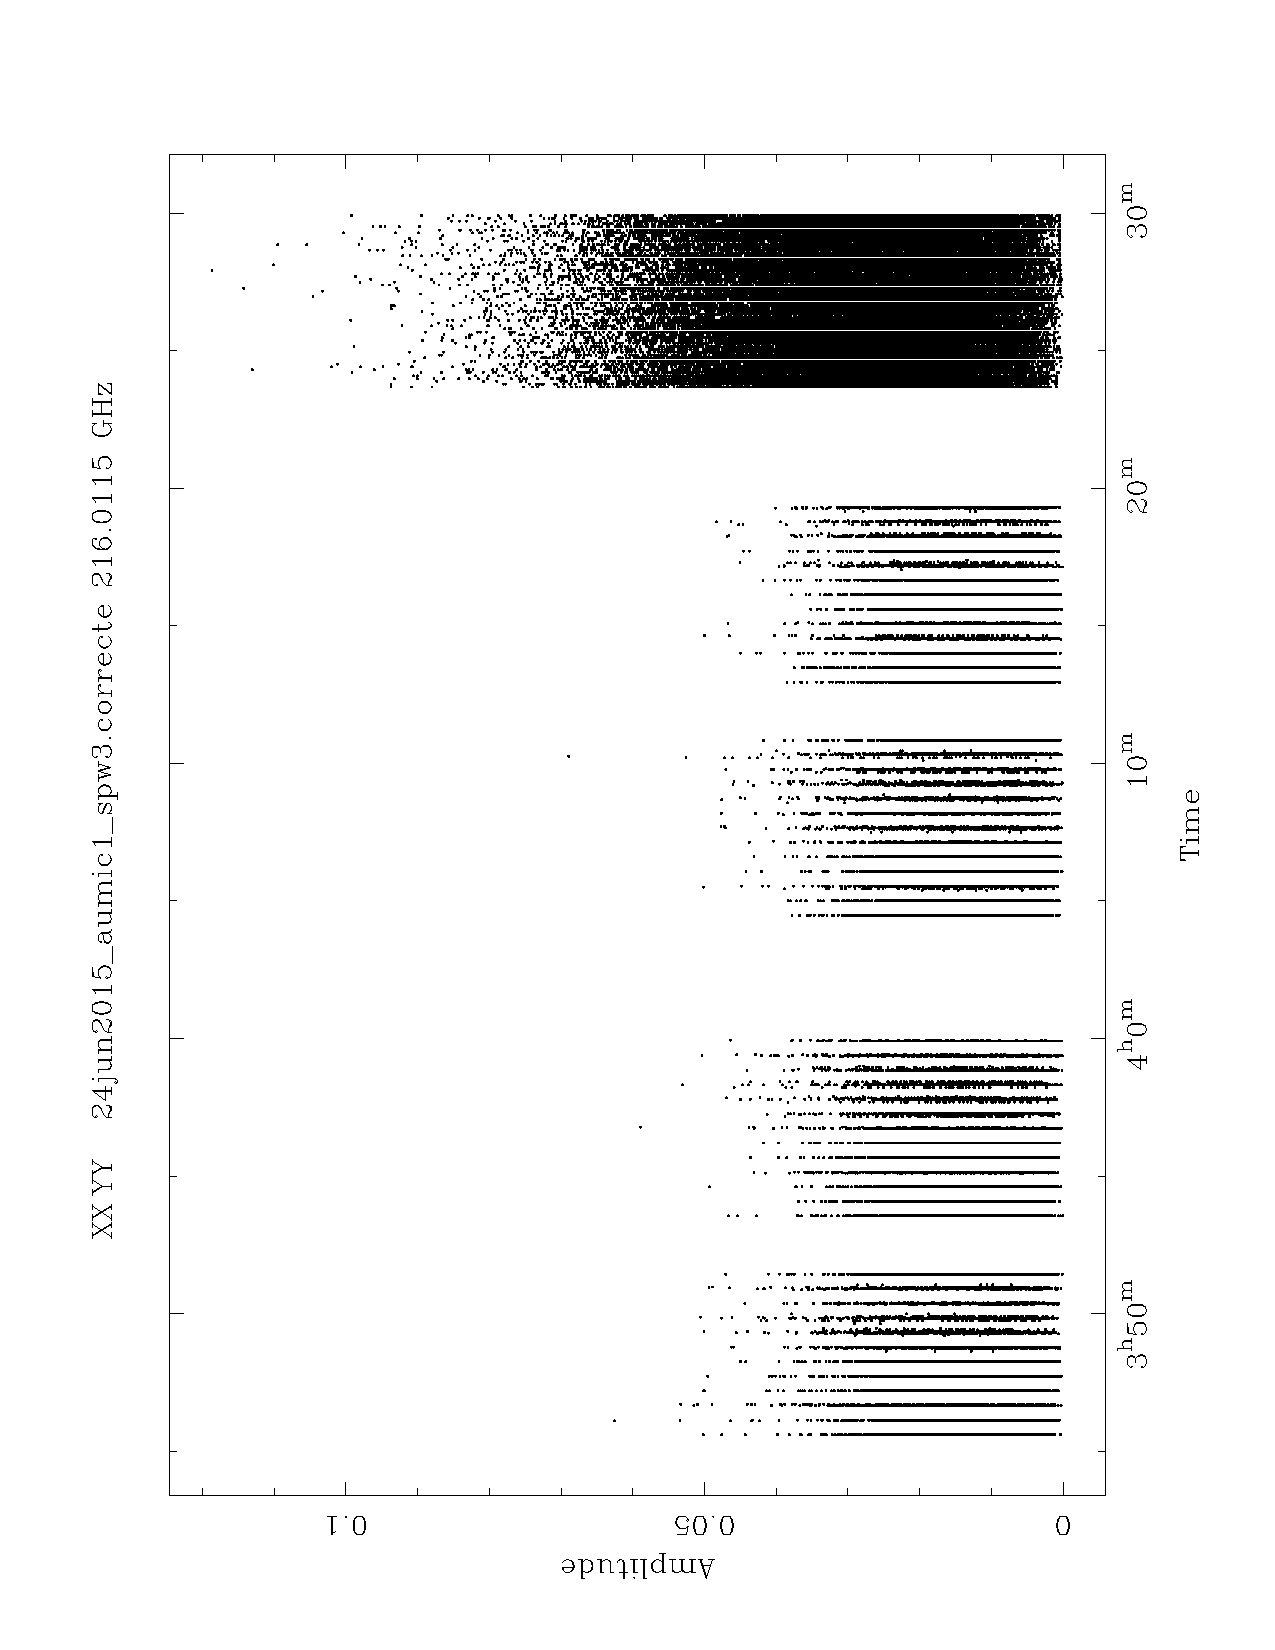
\includegraphics[width=.7\textwidth, angle=-90]{Figures/bad_vis_plot}
\end{figure}


\hrulefill
%%%%%%%%%%%%%%%%%%%%%%%%%%%%%%%%%%%%%%%%%%%%%%%%%%%%%%%%

\newday{18 November 2016}

\paragraph{Weights} \ \\
While looking at Kevin's weight correction code, Meredith and I realized that the code only calculates the weights for the \textit{real} component of the visibilities, and does not calculate the imaginary weights. As such, I was applying the real weights to both the real and imaginary visiblities to obtain the $\chi^2$ for my models. This is a decent approximation assuming that the real weights are roughly the same as the imaginary weights, i.e. \textbf{that the real dispersion is roughly the same as the imaginary dispersion}. However, plotting the real weight vs. the imaginary weights implies that this is not the case, and regardless some accuracy is lost using this approximation. Instead, we are calculating the total weight for each point as
\begin{align}
	\label{weight}
	wt_{tot} = \sqrt{wt_{real}wt_{imaginary}}
\end{align}
and inserting the total weights into both the xx and yy polarization columns of each data file.\\
When calculating the corrected weights for each file using the method described above, the code prints the mean absolute difference between the real and imaginary weights, defined as
\begin{align*}
	\mu_{diff} = \frac{\sum |wt_{real}-wt_{imaginary}|}{N}
\end{align*}

The values for $\mu_{diff}$, as well as $\chi^2$s calculated with the corrected weights, are tabulated below.

\begin{tabular}{lrr}
	\toprule
	File                     & Reduced $\chi^2$ & $\mu_{diff}$      \\
	\midrule
	18aug2015\_spw0          & 2.04             & \num{2777.94}     \\
	18aug2015\_spw1          & 2.04             & 3262.7            \\
	18aug2015\_spw2          & 2.04             & 3354.83           \\
	18aug2015\_spw3          & 2.05             & 3136.28           \\
	\textbf{24jun2015\_spw0} & 2.12             & \num{1.04171e+06} \\
	24jun2015\_spw1          & 1.99             & 963318.0          \\
	24jun2015\_spw2          & 2.01             & \num{1.26727e+06} \\
	\textbf{24jun2015\_spw3} & 12.18            & \num{2.39607e+08} \\
	26mar2014\_spw0          & 2.07             & 4755.47           \\
	26mar2014\_spw1          & 2.07             & 5064.5            \\
	26mar2014\_spw2          & 2.06             & 5180.01           \\
	26mar2014\_spw3          & 2.07             & 4431.92           \\
	\bottomrule
\end{tabular}

Using Equation \ref{weight} reduced the reduced $\chi^2$s for the bad spectral windows--this implies that the previously un-included imaginary weights tend to be smaller than the real weights. Kevin's weight correcting code also took about a factor of ten longer to run for the June date than for either of the other two.

\hrulefill
%%%%%%%%%%%%%%%%%%%%%%%%%%%%%%%%%%%%%%%%%%%%%%%%%%%%%%%%
\newday{1 November 2016}

\begin{itemize}
	\item Made sure that Modeling\_Code\_check.py deletes existing .vis files before it remakes them to avoid overwrite failure.
	\item Began setting up check code to do the splitting through miriad, rather than CASA-- hopefully I can use the weights created by Kevin's code for the miriad-split visibilities.
\end{itemize}


\hrulefill
%%%%%%%%%%%%%%%%%%%%%%%%%%%%%%%%%%%%%%%%%%%%%%%%%%%%%%%%
\newday{25 October 2016}

Created a new directory in AU\_Mic titled ``fixing\_spws'' to hold things related to fixing bad spws.\\
\indent Created a specialized version of my modeling code, Modeling\_Code\_check.py, to check $\chi^2$ for different spw splits.

\begin{itemize}
	\item Splitting 24 Jun spws 2 and 3 (one good spw and one bad one) by time to compare $\chi^2$
	\item NOTE: Can just use exportuvfits to split
\end{itemize}


% \hrulefill
%%%%%%%%%%%%%%%%%%%%%%%%%%%%%%%%%%%%%%%%%%%%%%%%%%%%%%%%

% \bibliographystyle{unsrt}
% \bibliography{aumic_notes}

\end{document}
